% Options for packages loaded elsewhere
\PassOptionsToPackage{unicode}{hyperref}
\PassOptionsToPackage{hyphens}{url}
\PassOptionsToPackage{dvipsnames,svgnames,x11names}{xcolor}
%
\documentclass[
  letterpaper,
  DIV=11,
  numbers=noendperiod]{scrreprt}

\usepackage{amsmath,amssymb}
\usepackage{iftex}
\ifPDFTeX
  \usepackage[T1]{fontenc}
  \usepackage[utf8]{inputenc}
  \usepackage{textcomp} % provide euro and other symbols
\else % if luatex or xetex
  \usepackage{unicode-math}
  \defaultfontfeatures{Scale=MatchLowercase}
  \defaultfontfeatures[\rmfamily]{Ligatures=TeX,Scale=1}
\fi
\usepackage{lmodern}
\ifPDFTeX\else  
    % xetex/luatex font selection
\fi
% Use upquote if available, for straight quotes in verbatim environments
\IfFileExists{upquote.sty}{\usepackage{upquote}}{}
\IfFileExists{microtype.sty}{% use microtype if available
  \usepackage[]{microtype}
  \UseMicrotypeSet[protrusion]{basicmath} % disable protrusion for tt fonts
}{}
\makeatletter
\@ifundefined{KOMAClassName}{% if non-KOMA class
  \IfFileExists{parskip.sty}{%
    \usepackage{parskip}
  }{% else
    \setlength{\parindent}{0pt}
    \setlength{\parskip}{6pt plus 2pt minus 1pt}}
}{% if KOMA class
  \KOMAoptions{parskip=half}}
\makeatother
\usepackage{xcolor}
\setlength{\emergencystretch}{3em} % prevent overfull lines
\setcounter{secnumdepth}{-\maxdimen} % remove section numbering
% Make \paragraph and \subparagraph free-standing
\ifx\paragraph\undefined\else
  \let\oldparagraph\paragraph
  \renewcommand{\paragraph}[1]{\oldparagraph{#1}\mbox{}}
\fi
\ifx\subparagraph\undefined\else
  \let\oldsubparagraph\subparagraph
  \renewcommand{\subparagraph}[1]{\oldsubparagraph{#1}\mbox{}}
\fi

\usepackage{color}
\usepackage{fancyvrb}
\newcommand{\VerbBar}{|}
\newcommand{\VERB}{\Verb[commandchars=\\\{\}]}
\DefineVerbatimEnvironment{Highlighting}{Verbatim}{commandchars=\\\{\}}
% Add ',fontsize=\small' for more characters per line
\usepackage{framed}
\definecolor{shadecolor}{RGB}{241,243,245}
\newenvironment{Shaded}{\begin{snugshade}}{\end{snugshade}}
\newcommand{\AlertTok}[1]{\textcolor[rgb]{0.68,0.00,0.00}{#1}}
\newcommand{\AnnotationTok}[1]{\textcolor[rgb]{0.37,0.37,0.37}{#1}}
\newcommand{\AttributeTok}[1]{\textcolor[rgb]{0.40,0.45,0.13}{#1}}
\newcommand{\BaseNTok}[1]{\textcolor[rgb]{0.68,0.00,0.00}{#1}}
\newcommand{\BuiltInTok}[1]{\textcolor[rgb]{0.00,0.23,0.31}{#1}}
\newcommand{\CharTok}[1]{\textcolor[rgb]{0.13,0.47,0.30}{#1}}
\newcommand{\CommentTok}[1]{\textcolor[rgb]{0.37,0.37,0.37}{#1}}
\newcommand{\CommentVarTok}[1]{\textcolor[rgb]{0.37,0.37,0.37}{\textit{#1}}}
\newcommand{\ConstantTok}[1]{\textcolor[rgb]{0.56,0.35,0.01}{#1}}
\newcommand{\ControlFlowTok}[1]{\textcolor[rgb]{0.00,0.23,0.31}{#1}}
\newcommand{\DataTypeTok}[1]{\textcolor[rgb]{0.68,0.00,0.00}{#1}}
\newcommand{\DecValTok}[1]{\textcolor[rgb]{0.68,0.00,0.00}{#1}}
\newcommand{\DocumentationTok}[1]{\textcolor[rgb]{0.37,0.37,0.37}{\textit{#1}}}
\newcommand{\ErrorTok}[1]{\textcolor[rgb]{0.68,0.00,0.00}{#1}}
\newcommand{\ExtensionTok}[1]{\textcolor[rgb]{0.00,0.23,0.31}{#1}}
\newcommand{\FloatTok}[1]{\textcolor[rgb]{0.68,0.00,0.00}{#1}}
\newcommand{\FunctionTok}[1]{\textcolor[rgb]{0.28,0.35,0.67}{#1}}
\newcommand{\ImportTok}[1]{\textcolor[rgb]{0.00,0.46,0.62}{#1}}
\newcommand{\InformationTok}[1]{\textcolor[rgb]{0.37,0.37,0.37}{#1}}
\newcommand{\KeywordTok}[1]{\textcolor[rgb]{0.00,0.23,0.31}{#1}}
\newcommand{\NormalTok}[1]{\textcolor[rgb]{0.00,0.23,0.31}{#1}}
\newcommand{\OperatorTok}[1]{\textcolor[rgb]{0.37,0.37,0.37}{#1}}
\newcommand{\OtherTok}[1]{\textcolor[rgb]{0.00,0.23,0.31}{#1}}
\newcommand{\PreprocessorTok}[1]{\textcolor[rgb]{0.68,0.00,0.00}{#1}}
\newcommand{\RegionMarkerTok}[1]{\textcolor[rgb]{0.00,0.23,0.31}{#1}}
\newcommand{\SpecialCharTok}[1]{\textcolor[rgb]{0.37,0.37,0.37}{#1}}
\newcommand{\SpecialStringTok}[1]{\textcolor[rgb]{0.13,0.47,0.30}{#1}}
\newcommand{\StringTok}[1]{\textcolor[rgb]{0.13,0.47,0.30}{#1}}
\newcommand{\VariableTok}[1]{\textcolor[rgb]{0.07,0.07,0.07}{#1}}
\newcommand{\VerbatimStringTok}[1]{\textcolor[rgb]{0.13,0.47,0.30}{#1}}
\newcommand{\WarningTok}[1]{\textcolor[rgb]{0.37,0.37,0.37}{\textit{#1}}}

\providecommand{\tightlist}{%
  \setlength{\itemsep}{0pt}\setlength{\parskip}{0pt}}\usepackage{longtable,booktabs,array}
\usepackage{calc} % for calculating minipage widths
% Correct order of tables after \paragraph or \subparagraph
\usepackage{etoolbox}
\makeatletter
\patchcmd\longtable{\par}{\if@noskipsec\mbox{}\fi\par}{}{}
\makeatother
% Allow footnotes in longtable head/foot
\IfFileExists{footnotehyper.sty}{\usepackage{footnotehyper}}{\usepackage{footnote}}
\makesavenoteenv{longtable}
\usepackage{graphicx}
\makeatletter
\def\maxwidth{\ifdim\Gin@nat@width>\linewidth\linewidth\else\Gin@nat@width\fi}
\def\maxheight{\ifdim\Gin@nat@height>\textheight\textheight\else\Gin@nat@height\fi}
\makeatother
% Scale images if necessary, so that they will not overflow the page
% margins by default, and it is still possible to overwrite the defaults
% using explicit options in \includegraphics[width, height, ...]{}
\setkeys{Gin}{width=\maxwidth,height=\maxheight,keepaspectratio}
% Set default figure placement to htbp
\makeatletter
\def\fps@figure{htbp}
\makeatother
% definitions for citeproc citations
\NewDocumentCommand\citeproctext{}{}
\NewDocumentCommand\citeproc{mm}{%
  \begingroup\def\citeproctext{#2}\cite{#1}\endgroup}
\makeatletter
 % allow citations to break across lines
 \let\@cite@ofmt\@firstofone
 % avoid brackets around text for \cite:
 \def\@biblabel#1{}
 \def\@cite#1#2{{#1\if@tempswa , #2\fi}}
\makeatother
\newlength{\cslhangindent}
\setlength{\cslhangindent}{1.5em}
\newlength{\csllabelwidth}
\setlength{\csllabelwidth}{3em}
\newenvironment{CSLReferences}[2] % #1 hanging-indent, #2 entry-spacing
 {\begin{list}{}{%
  \setlength{\itemindent}{0pt}
  \setlength{\leftmargin}{0pt}
  \setlength{\parsep}{0pt}
  % turn on hanging indent if param 1 is 1
  \ifodd #1
   \setlength{\leftmargin}{\cslhangindent}
   \setlength{\itemindent}{-1\cslhangindent}
  \fi
  % set entry spacing
  \setlength{\itemsep}{#2\baselineskip}}}
 {\end{list}}
\usepackage{calc}
\newcommand{\CSLBlock}[1]{\hfill\break\parbox[t]{\linewidth}{\strut\ignorespaces#1\strut}}
\newcommand{\CSLLeftMargin}[1]{\parbox[t]{\csllabelwidth}{\strut#1\strut}}
\newcommand{\CSLRightInline}[1]{\parbox[t]{\linewidth - \csllabelwidth}{\strut#1\strut}}
\newcommand{\CSLIndent}[1]{\hspace{\cslhangindent}#1}

\KOMAoption{captions}{tableheading}
\makeatletter
\@ifpackageloaded{caption}{}{\usepackage{caption}}
\AtBeginDocument{%
\ifdefined\contentsname
  \renewcommand*\contentsname{Table of contents}
\else
  \newcommand\contentsname{Table of contents}
\fi
\ifdefined\listfigurename
  \renewcommand*\listfigurename{List of Figures}
\else
  \newcommand\listfigurename{List of Figures}
\fi
\ifdefined\listtablename
  \renewcommand*\listtablename{List of Tables}
\else
  \newcommand\listtablename{List of Tables}
\fi
\ifdefined\figurename
  \renewcommand*\figurename{Figure}
\else
  \newcommand\figurename{Figure}
\fi
\ifdefined\tablename
  \renewcommand*\tablename{Table}
\else
  \newcommand\tablename{Table}
\fi
}
\@ifpackageloaded{float}{}{\usepackage{float}}
\floatstyle{ruled}
\@ifundefined{c@chapter}{\newfloat{codelisting}{h}{lop}}{\newfloat{codelisting}{h}{lop}[chapter]}
\floatname{codelisting}{Listing}
\newcommand*\listoflistings{\listof{codelisting}{List of Listings}}
\makeatother
\makeatletter
\makeatother
\makeatletter
\@ifpackageloaded{caption}{}{\usepackage{caption}}
\@ifpackageloaded{subcaption}{}{\usepackage{subcaption}}
\makeatother
\ifLuaTeX
  \usepackage{selnolig}  % disable illegal ligatures
\fi
\usepackage{bookmark}

\IfFileExists{xurl.sty}{\usepackage{xurl}}{} % add URL line breaks if available
\urlstyle{same} % disable monospaced font for URLs
\hypersetup{
  colorlinks=true,
  linkcolor={blue},
  filecolor={Maroon},
  citecolor={Blue},
  urlcolor={Blue},
  pdfcreator={LaTeX via pandoc}}

\author{}
\date{}

\begin{document}

\chapter{Reproducible Documents}\label{reproducible-documents}

\section{Why do we need reproducible
documents?}\label{why-do-we-need-reproducible-documents}

Traditional workflows within science use many different kinds of tools.
This requires careful recording of what happens at each step of the
scientific process. Good laboratory notebook practices are a feature of
many sciences but are not typically taught as part of a psychology
curriculum. This combination within psychology of a lack of clear
recording of data collection and analysis practices can lead to
difficulties in retracing the steps that led to any given outcome in
science. A traditional workflow in psychology may involve the design of
research and preparation for ethical review using a word processor and
perhaps some diagramming tools. This is followed by data collection on a
different platform perhaps using pen and paper in a laboratory, but
increasingly using automated platforms such as Qualtrics, PsychoPy, or
jsPsych. Following this data is manipulated from the shape it comes from
the platform and is wrangled into the right shape for analysis sometimes
in a statistical program, but often using cut and paste techniques in
Microsoft Excel or a similar spreadsheet program. The data is then
analysed using some statistical software platform such SPSS, SAS, JASP,
Jamovi or R. When the results are found these are extracted and the
whole sequence is written up using some combination of a word
processor---typically Microsoft Word---and perhaps some citation
software such as Endnote or RefWorks.

The problem with this approach is that it is not very reproducible, the
steps are difficult to trace unless the researcher is inordinately
meticulous with their recording and it is prone to untraceable errors.

The solution is to create a reproducible document.

\section{What are reproducible
documents?}\label{what-are-reproducible-documents}

Reproducible documents are a way of eliminating as many of these
disparate steps as possible and maximising the recording of the steps
that are taken along the research process. The goal is to streamline the
research process while making it more transparent and reproducible.
Ideally these documents will be made available for the scrutiny of other
scientific researchers and the public, but there are many advantages to
using reproducible documents as they make the process of conducting
science more efficient and they make research much easier to pick up
after the inevitable six month to year hiatuses that occur throughout
the scientific process as projects go through their different stages and
the myriad competing attention drawing factors of a professional
researchers life fragment our time.

We are not yet at a stage where all of the various platforms and
processes can be accumulated into one work flow but we can do much
better than the traditional approach.

Typically a reproducible document is a combination of some word
processing tools to create the document with mechanisms to insert
computer code chunks that allow us to load, store, and manipulate data;
conduct statistical and mathematical analysis; visualise the analysis
producing tables and plots as part of the document output; and
integrating with citation software to allow the easy creation of
references.

\section{The tools of reproducible
documents}\label{the-tools-of-reproducible-documents}

\subsection{Document preparation
tools}\label{document-preparation-tools}

There are a range of preexisting computational technologies that can be
brought together to enable these documents. The TeX and LaTeX systems
are well established document preparation and typesetting systems
(\href{https://www.latex-project.org}{latex-project}), these are aided
by the use of Markdown
(\href{https://www.markdownguide.org}{markdownguide.org}) which provides
a very simple document markup language which the researcher uses to
create the documents and pandoc (\href{https://pandoc.org}{pandoc.org})
which allows the same markdown document to be output to many different
formats. One markdown document can be used to create websites, PDFs,
Word documents, ePub books and many more. These represent the word
processing part.

\subsection{Code chunks}\label{code-chunks}

The computer chunks are comprised of various different languages that
can be mixed and matched, the most commonly used languages are R and
Python, but languages like Julia, Stan, Javascript, SQL, C, and Fortran.

The current document is being written as a reproducible document using
the RStudio software and I can include a code chunk in R

\begin{Shaded}
\begin{Highlighting}[]
\NormalTok{data }\OtherTok{\textless{}{-}} \FunctionTok{c}\NormalTok{(}\DecValTok{1}\NormalTok{,}\DecValTok{2}\NormalTok{,}\DecValTok{3}\NormalTok{,}\DecValTok{4}\NormalTok{,}\DecValTok{5}\NormalTok{,}\DecValTok{6}\NormalTok{,}\DecValTok{7}\NormalTok{,}\DecValTok{8}\NormalTok{,}\DecValTok{9}\NormalTok{,}\DecValTok{10}\NormalTok{)}
\NormalTok{x }\OtherTok{\textless{}{-}} \FunctionTok{mean}\NormalTok{(data)}
\FunctionTok{print}\NormalTok{(x)}
\end{Highlighting}
\end{Shaded}

\begin{verbatim}
[1] 5.5
\end{verbatim}

or in python

\begin{Shaded}
\begin{Highlighting}[]
\ImportTok{import}\NormalTok{ statistics}
\NormalTok{data }\OperatorTok{=}\NormalTok{ [}\DecValTok{1}\NormalTok{,}\DecValTok{2}\NormalTok{,}\DecValTok{3}\NormalTok{,}\DecValTok{4}\NormalTok{,}\DecValTok{5}\NormalTok{,}\DecValTok{6}\NormalTok{,}\DecValTok{7}\NormalTok{,}\DecValTok{8}\NormalTok{,}\DecValTok{9}\NormalTok{,}\DecValTok{10}\NormalTok{]}
\NormalTok{x }\OperatorTok{=}\NormalTok{ statistics.mean(data)}
\BuiltInTok{print}\NormalTok{(x)}
\end{Highlighting}
\end{Shaded}

\begin{verbatim}
5.5
\end{verbatim}

Code chunks can be hidden and only the output produced which is useful
when including any data wrangling code that you do not want to be seen
in a finished output, of for creating tables and plots. The important
thing is that the code remains visible in the source form of the
document so it can be inspected if necessary and it stays in the one
place with the end product document. You can see this process at work in
Figure~\ref{fig-airquality}, which contains code included in the source
document but hidden in the final document.

\begin{figure}

\centering{

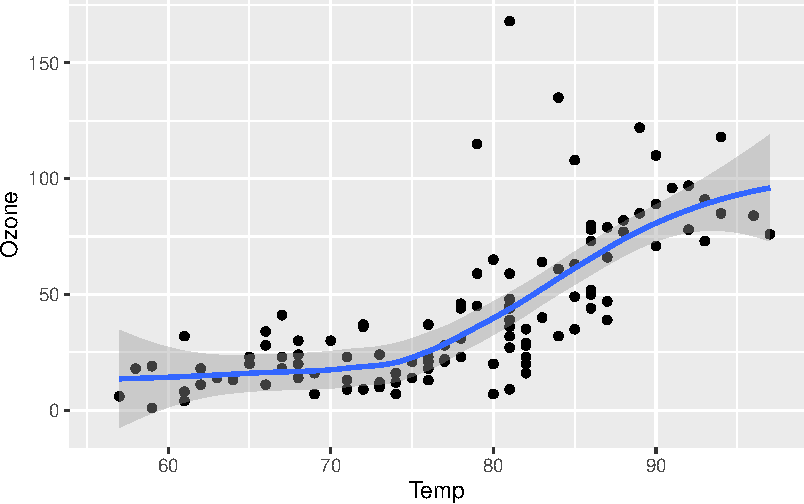
\includegraphics{reproducible_documents_files/figure-pdf/fig-airquality-1.pdf}

}

\caption{\label{fig-airquality}Temperature and ozone level.}

\end{figure}%

\subsection{Citation software}\label{citation-software}

Citation management and the automatic creation of a references section
are important components of reproducible document systems. Most systems
interact with pandoc, BibTeX, Zotero, Crossref, PubMed, and the DOI
system to allow in text citations with automated References sections
(e.g. McKeown, 2013). This reference will appear in the References
section automatically without any more work.

\subsection{Version control}\label{version-control}

An important but optional companion technology to the creation of
reproducible documents is the variety of version control software such
as git or svn. Git is the currently most popular type of version
control. Version control systems were developed to keep track of the
various changes that were made to computer code and to allow variations
of code to be made and merged into a single document and to allow
collaboration by multiple coders without the danger of overwriting each
other. This turns out to be handy when it comes to writing documents
too, especially documents that contain code. Think of version control as
a high powered and rigorous combination of ``track changes'' and backing
up files. It is a solution to folders full of final final final versions
of the same document. Git is a piece of software that sits on your local
computer and controls the versions of your documents, but it has a
companion in github that offers remote hosting of documents and enables
collaboration between multiple contributors. You can see the code for
this document at
(\href{https://github.com/QUBPsy/QUBPsyOpenScience}{github.com/QUBPsy/QUBPsyOpenScience}).

\section{Reproducible Document
Platforms}\label{reproducible-document-platforms}

There are a variety of ways of creating reproducible documents. Here we
will look at some of the options.

\subsection[ RStudio and R
Markdown]{\texorpdfstring{\protect
\includegraphics[width=0.625in,height=\textheight]{images/RStudio.png}\protect
\includegraphics[width=0.625in,height=\textheight]{images/rmarkdownlogo.png}
RStudio and R
Markdown}{ RStudio and R Markdown}}\label{rstudio-and-r-markdown}

One of the two major pioneers of mechanisms to produce reproducible
documents came from the combination of the R focused Integrated
Development Environment (IDE) RStudio. RStudio started in 2011 to create
an easy environment in which to write R code and install and manage R
packages. In 2012 Yihui Xie introduced the knitr package to enable the
creation of documents with code chunks embedded in them. Markdown become
the most popular language to develop these documents and the rmarkdown
package was introduced in 2014, and it became well embedded within the
RSTudio IDE where a lot of effort was made to make the production of
RMarkdown documents simple and easy. The kinds of documents that could
be produced in RMarkdown, webpages and websites, pdf documents, Shiny
web apps, journal articles, slides and presentations, and books.

The R Markdown ecosystem is now quite mature and there are many packages
that allow people to get up and running with many different aspects such
as: the creation of quite sophisticated websites using RStudio and
Github pages (with many other options); the creation of APA style
manuscripts and journal articles using
\href{http://frederikaust.com/papaja_man/}{papaja} (although this
remains somewhat buggy); templates to aid in the creation of many
different kinds of journal articles through rticles such as Elsevier,
IEEE, Royal Society, Springer, PNAS journal templates
(Table~\ref{tbl-rticlesjournals} provides a full list of journal
abbreviations); full book creation in online, pdf and ePub formats using
\href{https://bookdown.org}{bookdown} (see an example
\href{https://bookdown.org/yihui/rmarkdown/}{here}); various kinds of
presentations (Powerpoint, Beamer, Slidy); dashboards using the
flexdashboard package; and interactive documents incorporating Shiny web
apps and html widgets.

\begin{longtable}[]{@{}ccc@{}}

\caption{\label{tbl-rticlesjournals}The abbreviations for the R Markdown
journal article templates avaialble in the rticles R package.}

\tabularnewline

\toprule\noalign{}
\endhead
\bottomrule\noalign{}
\endlastfoot
acm & frontiers & oup\_v0 \\
acs & glossa & oup\_v1 \\
aea & ieee & peerj \\
agu & ims & pihph \\
ajs & informs & plos \\
amq & iop & pnas \\
ams & isba & rjournal \\
arxiv & jasa & rsos \\
asa & jedm & rss \\
bioinformatics & joss & sage \\
biometrics & jss & sim \\
copernicus & lipics & springer \\
ctex & lncs & tf \\
elsevier & mdpi & trb \\

\end{longtable}

One issue that arises with reproducible documents arises due to their
instrinsic nature; they contain code. Code depends on other code and
code changes with time. There are constant updates to packages and
software and often these updates will break older code as functions
become deprecated or change in nature. The solution to this problem is
to create environments in which to encapsulate code and its
dependencies. In R the
\href{https://rstudio.github.io/packrat/}{Packrat} and newer
\href{https://rstudio.github.io/renv/articles/renv.html}{renv} packages
are designed to provide this dependency management within R. These
packages will create a local environment snapshot of all the necessary
code and allow them to reloaded whent he time comes to work with the
files. An example of a reproducible document that uses renv to do this
can be found at
\href{https://github.com/damien-dupre/machine_challenge}{this github
repository} which provided the code to produce and run all the
experiments need to produce this paper (Dupré et al., 2020).

\subsection[ JupyterLab, Jupyter Notebooks and
Python]{\texorpdfstring{\protect
\includegraphics[width=0.625in,height=\textheight]{images/squarelogo-greytext-orangebody-greymoons.png}
JupyterLab, Jupyter Notebooks and
Python}{ JupyterLab, Jupyter Notebooks and Python}}\label{jupyterlab-jupyter-notebooks-and-python}

Another option for creating reproducible documents that has its origins
in the Python computer language ecosystem is Jupyter Notebooks.
Typically these require knowledge of the Python programming language and
comfort working in a command line environment such as terminals in Unix
environments and Windows Terminal in Windows 10 and above (previously
the Windows Console).

A Jupyter Notebook is a reproducible document that normally sits in a
folder on your computer and you interact with using an interface in your
browser. You navigate to the appropriate folder in your terminal and
type ``jupyter notebook'' and this opens your browser and browser window
that allows you to interact with the document. Documents contain a mix
of text and code. The is a classic Jupyter Notebook interface and a more
advanced IDE style interface known as JupyterLab. There are online
servers that will allow you to interact with Jupyter Notebooks without
the need to install software and have a dedicated machine, some of these
can be seen at the Jupyter project:
\href{https://jupyter.org/try-jupyter/retro/notebooks/?path=notebooks/Intro.ipynb}{classic
interface}, \href{https://jupyter.org/try-jupyter/lab/}{JupyterLab
interface}. Similarly to RStudio even though they started firmly focused
on one language---Python---but they also realised the value in
supporting multiple languages and allowing them to be used
interchangeably, they now support about 40 languages including R
(\href{https://mybinder.org/v2/gh/binder-examples/r/HEAD?filepath=index.ipynb}{R
in a Jupyter Notebook}).

Dependency issues in Python can be dealt with in a similar way to R by
creating environments in which the code and packages can be isolated
from other environments. The use of virtual environments in Python is
more well established than in R and there are a variety of ways to
create them. For example, the
\href{https://docs.python.org/3/library/venv.html}{venv} module, the
\href{https://pypi.org/project/virtualenv/}{virtualenv} package, or
within the
\href{https://docs.conda.io/projects/conda/en/latest/user-guide/tasks/manage-environments.html}{Anaconda
Python distribution platform}. Virtual environments are often advised as
best practice within general Python usage.

\subsection[Quarto]{\texorpdfstring{\protect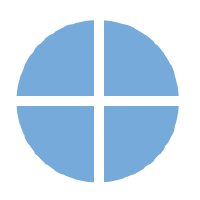
\includegraphics[width=0.625in,height=\textheight]{images/Quartologo.png}Quarto}{Quarto}}\label{quarto}

The two previous reproducible document approaches showed a trend from
focusing on a single language towards reproducible documents that are
more flexible. Recently the people at RStudio have announced that they
have taken this a step further with the development of
\href{https://quarto.org}{Quarto}, Quarto is a reproducible document
system again built on Pandoc allowing documents to be created using
Markdown or Jupyter Notebooks. Quarto is installed independently of the
other systems as separate software on the computer and then each of the
systems interface with it. Reproducible documents can then be created in
a text editor, RStudio, Jupyter Notebooks or VS Code (Microsoft's Visual
Studio Code IDE). The goal is to make the document production part of
the system agnostic to the way in which people prefer to work. As it is
being spearheaded by RStudio it is likely to supersede the current R
Markdown ecosystem (although R Markdown will be around for a long time).
In producing Quarto the Rstudio team have taken the opportunity to make
some of the issues that existed with R Markdown better and they seek to
make a more unified system for developing each of the different styles
of output. It is still in its infancy but I expect that it will quickly
become the standard within the R ecosystem at least. This current
book/website hybrid has been created using Quarto, although it's very
first incarnation was as a R Markdown Bookdown project.

\subsection[ VS
Code]{\texorpdfstring{\protect
\includegraphics[width=0.625in,height=\textheight]{images/vscode_icon.png}
VS Code}{ VS Code}}\label{vs-code}

Microsoft's Visual Studio Code is an IDE that is used by many people who
do development within the Windows ecosystem. With the arrival of Quarto
it can now be used as an environment for developing reproducible
documents. It requires the addition of a Code Extension. This may be
useful if you are already a user of VS Code otherwise the Rstudio IDE is
probably a better place to start.

\phantomsection\label{refs}
\begin{CSLReferences}{1}{0}
\bibitem[\citeproctext]{ref-dupruxe92020}
Dupré, D., Krumhuber, E. G., Küster, D., \& McKeown, G. J. (2020). A
performance comparison of eight commercially available automatic
classifiers for facial affect recognition. \emph{PLOS ONE},
\emph{15}(4), e0231968.
\url{https://doi.org/10.1371/journal.pone.0231968}

\bibitem[\citeproctext]{ref-mckeown2013}
McKeown, G. J. (2013). The Analogical Peacock Hypothesis: The Sexual
Selection of Mind-Reading and Relational Cognition in Human
Communication. \emph{Review of General Psychology}, \emph{17}(3),
267--287. \url{https://doi.org/10.1037/a0032631}

\end{CSLReferences}



\end{document}
